\section{Basics}

\subsection{What is a widget?}

\begin{frame}{Everything is a widget}
    The core of Flutter's layout mechanism is widgets.

    They describe what their view should look like given their current configuration and state.

    When a widget's state changes, the widget rebuilds its description, which the framework diffs against the previous description in order to determine the minimal changes needed in the underlying render tree to transition from one state to the next.
\end{frame}

\begin{frame}{Everything is a widget}
    How many widgets here?
    \begin{figure}[h]
        
\includegraphics[width=0.4\textwidth]{images/lakes-icons.png}<1->
    \end{figure}

    \begin{figure}[h]
        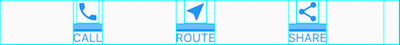
\includegraphics[width=0.4\textwidth]{images/lakes-icons-visual.png}<2->
    \end{figure}

    \only<3->{14 widgets!}
\end{frame}

\begin{frame}{Everything is a widget}
    \begin{figure}[h]
        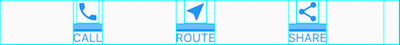
\includegraphics[width=0.4\textwidth]{images/lakes-icons-visual.png}
    \end{figure}
    \begin{figure}[h]
        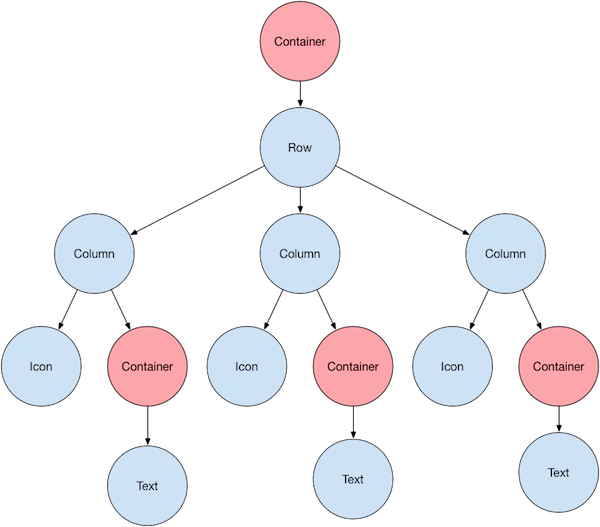
\includegraphics[width=0.6\textwidth]{images/sample-flutter-layout.png}
    \end{figure}
\end{frame}

\subsection{What is State?}

\begin{frame}{What is State?}
    \begin{block}{State}
        Information that can be read synchronously when the widget is built and might change during the lifetime of the widget.
    \end{block}
\end{frame}

\subsection{Types of widgets}
\begin{frame}{Types of widgets}

There are 2 types of widgets:

\begin{block}{Stateless Widgets}<2>
    They do not own a mutable state.

    Useful when the part of the user interface you are describing does not depend on anything other than the configuration information in the object itself and the context in which the widget is inflated.
\end{block}
    
\end{frame}

\begin{frame}{Types of widgets}
    
    There are 2 types of widgets:
    
    \begin{block}{Stateful Widgets}
        They are themselves immutable. However, they own a State.
        
        Useful when the part of the user interface you are describing can change dynamically, e.g. due to having an internal clock-driven state or depending on some system state
    \end{block}
    
\end{frame}

\subsection{Widget Lifecycle}
\begin{frame}{Widget Lifecycle}
    \begin{figure}[h]
        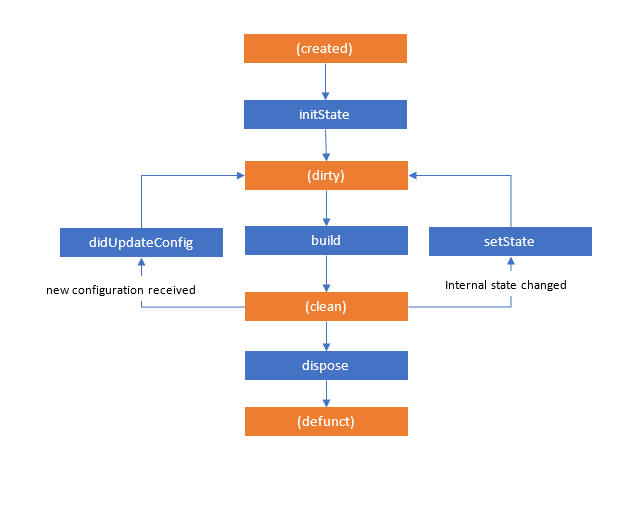
\includegraphics[width=0.8\textwidth]{images/lifecycle.png}
    \end{figure}
\end{frame}